\documentclass[conference]{IEEEtran}
\IEEEoverridecommandlockouts
%Template version as of 6/27/2024

\usepackage[utf8]{inputenc}
% es-nodecimaldot: sin esto, babel-spanish convierte el punto decimal en coma
% dentro de modo matemático, y las tablas mezclan "-14,7187" con "0.3253".
\usepackage[spanish,es-nodecimaldot]{babel}
\usepackage{cite}
\usepackage{amsmath,amssymb,amsfonts}
\usepackage{algorithmic}
\usepackage{graphicx}
\graphicspath{{./}{report/}{modulo_2/linear-regression-from-scratch/report/}}
\usepackage{textcomp}
\usepackage{xcolor}
\usepackage{booktabs}
\usepackage{hyperref}
\def\BibTeX{{\rm B\kern-.05em{\sc i\kern-.025em b}\kern-.08em
    T\kern-.1667em\lower.7ex\hbox{E}\kern-.125emX}}
\begin{document}

\title{Implementación de Regresión Lineal Múltiple desde Cero mediante Descenso de Gradiente}

\author{\IEEEauthorblockN{Facundo Bautista Barbera}
\IEEEauthorblockA{\textit{Escuela de Ingeniería y Ciencias} \\
\textit{Instituto Tecnológico y de Estudios Superiores de Monterrey}\\
A01066843@tec.mx}
}

\maketitle

\begin{abstract}
Este reporte presenta un modelo de regresión lineal múltiple implementado con Python base y entrenado con gradiente descendente, sin el uso de frameworks o librerías de machine learning. El modelo está entrenado y evaluado en el dataset de ``Combined Cycle Power Plant'' del UCI Machine Learning Repository, el cual contiene 9,527 instancias que representan horas de la operación de la planta en su máxima capacidad, y predice la salida de energía eléctrica neta a partir de 4 variables ambientales. El reporte describe el proceso de limpieza de datos, las matemáticas del modelo, la estandarización de las variables de entrada y el proceso de selección automática de la velocidad de aprendizaje. El modelo resultante explica el 93.19\% de la varianza en el set de pruebas con $R^2$ de 0.9319 y RMSE de 4.43 MW, alcanzando coeficientes idénticos a los generados con una referencia de implementación con scikit-learn como método de comparación. Se documentó un proceso de validación cruzada, obteniendo un $R^2$ de $0.9283 \pm 0.0020$, confirmando que el resultado no depende de una partición particular. Un Random Forest entrenado con los mismos datos obtuvo un score más elevado, con $R^2$ de 0.9616. También se analizaron los efectos que tienen diferentes tasas de aprendizaje y número de épocas sobre la convergencia.
\end{abstract}

\begin{IEEEkeywords}
regresión lineal múltiple, descenso de gradiente, MSE, estandarización, aprendizaje máquina, Python, hiperparámetros
\end{IEEEkeywords}

\section{Introducción}
\label{sec:intro}
La regresión lineal es uno de los modelos fundamentales del machine learning supervisado, y es el punto de inicio para entender cómo un modelo aprende de los datos. Frameworks modernos como scikit-learn resuelven los problemas en una función, lo cual hace que sea muy fácil de aplicar pero esconde el proceso que realmente produce el resultado. Implementar el algoritmo sin librerías especializadas fuerza a uno a entender cada componente que esos frameworks abstraen: las funciones de hipótesis, las funciones de costo, el gradiente del costo con respecto a los parámetros, y las reglas que llevan a un modelo al óptimo. 

El objetivo de este trabajo es implementar un modelo de regresión lineal múltiple en Python base, es decir sin librerías externas ni frameworks, entrenarlo con gradiente descendente en un dataset real, y validar su comportamiento contra un punto de referencia. El problema que se seleccionó es la predicción de la salida de electricidad de una planta de energía usando variables que corresponden a las condiciones ambientales de operación.

El reporte está organizado de la siguiente forma: La sección~\ref{sec:dataset} describe el dataset y sus variables. La sección~\ref{sec:etl} cubre la extracción, limpieza y transformación de los datos. La sección~\ref{sec:modelo} presenta las matemáticas del modelo y su implementación. La sección~\ref{sec:resultados} reporta los resultados del caso base. La sección~\ref{sec:diagnostico} diagnostica el modelo en términos de sesgo y varianza. La sección~\ref{sec:comparacion} compara la implementación manual contra la de scikit-learn. La sección~\ref{sec:hiperparametros} analiza el efecto de hiperparámetros. Y la sección~\ref{sec:conclusiones} presenta las conclusiones.

\section{Descripción del dataset}
\label{sec:dataset}
Este estudio usa el dataset ``Combined Cycle Power Plant'' o CCPP, obtenido de UCI Machine Learning Repository, y tiene datos de 6 años (2006 a 2011) de una planta eléctrica operando a capacidad máxima. Cada instancia representa las condiciones de operación de la planta promediadas por hora, es decir cada instancia representa una hora promedio de operación, descrita por 4 variables de ambiente: ambient temperature (AT, °C), exhaust vacuum (V, cm Hg), ambient pressure (AP, mbar) y relative humidity (RH, \%), y la salida de energía eléctrica neta (PE, MW), la cual será nuestra variable objetivo. El archivo de datos contiene 9,568 instancias y 9,527 instancias después de limpiar. La Tabla~\ref{tab:descriptiva} tiene el resumen de las variables.

Las 4 variables ambientales se usan como features predictoras. La ambient temperature es la variable con más relación a la variable objetivo, con un valor de Pearson de -0.948, exhaust vacuum es la segunda variable más correlacionada con un valor de -0.870, ambas variables con una correlación negativa, es decir, si el valor de estas es más alto el resultado del modelo debería ser más bajo. Las variables ``ambient pressure'' (+0.519) y ``relative humidity'' (+0.391) contribuyen al modelo pero en un porcentaje menor y con relación positiva. La Figura~\ref{fig:correlacion} muestra la matriz de correlación completa, donde se observa que AT y V también están fuertemente correlacionadas entre sí (+0.844), ya que ambas reflejan el punto térmico de operación de la planta. La Figura~\ref{fig:histogramas} muestra la distribución de cada variable. Las relaciones dominantes son claramente lineales: una mayor temperatura de admisión reduce la eficiencia de la turbina, por lo que la planta genera menos potencia. Este comportamiento justifica modelar el problema con una regresión lineal múltiple.

\begin{table}[htbp]
\caption{Estadística descriptiva de las variables ($n = 9\,527$)}
\label{tab:descriptiva}
\centering
\begin{tabular}{lcccc}
\toprule
Variable & Media & Desv. est. & Mínimo & Máximo \\
\midrule
AT (\textdegree C) & 19.65 & 7.45 & 1.81 & 37.11 \\
V (cm Hg) & 54.31 & 12.71 & 25.36 & 81.56 \\
AP (mbar) & 1013.26 & 5.94 & 992.89 & 1033.30 \\
RH (\%) & 73.31 & 14.60 & 25.56 & 100.16 \\
PE (MW) & 454.37 & 17.07 & 420.26 & 495.76 \\
\bottomrule
\end{tabular}
\end{table}

\begin{figure}[htbp]
\centering
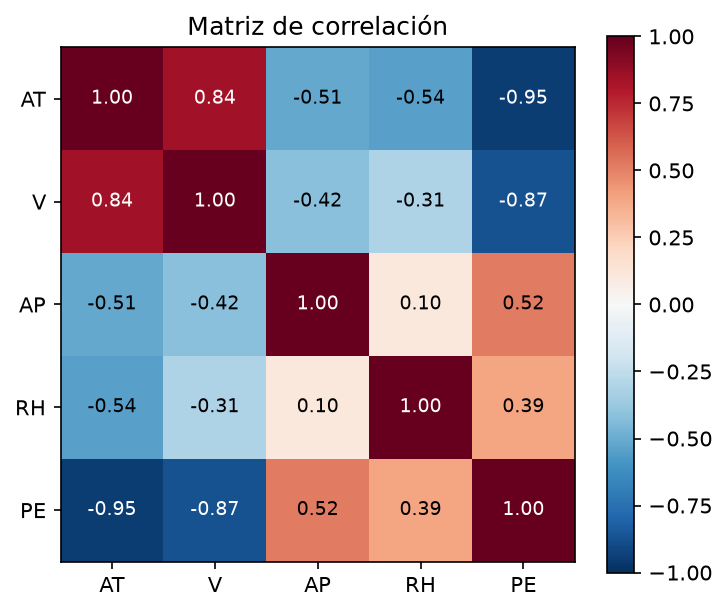
\includegraphics[width=\columnwidth]{figures/correlacion.png}
\caption{Matriz de correlación entre las variables.}
\label{fig:correlacion}
\end{figure}
\begin{figure}[htbp]
\centering
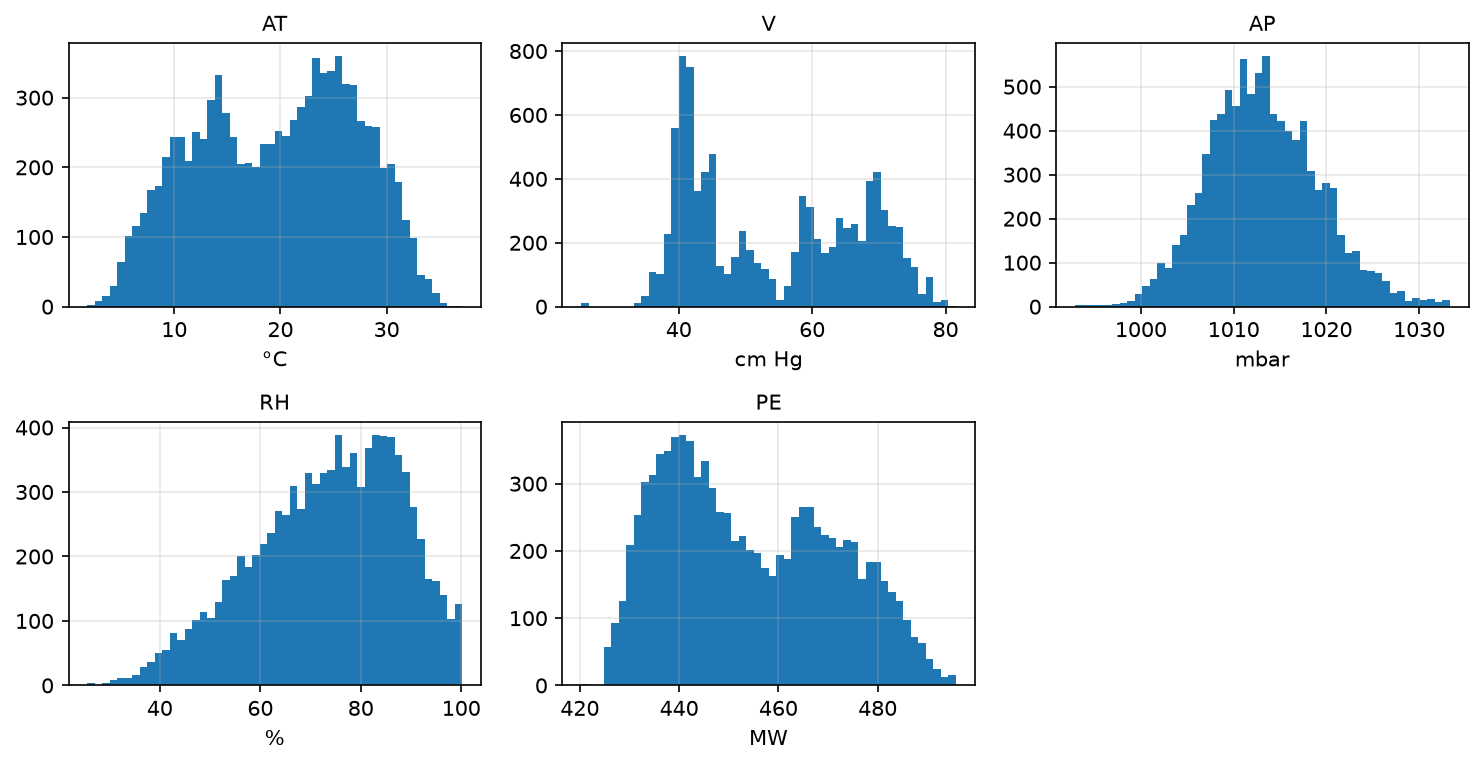
\includegraphics[width=\columnwidth]{figures/histogramas.png}
\caption{Distribución de cada variable del conjunto de datos.}
\label{fig:histogramas}
\end{figure}

\section{Extracción, limpieza y transformación de datos}
\label{sec:etl}
\subsection{Limpieza}
El dataset no contiene valores faltantes en ninguna de las 5 columnas, no hubo necesidad de hacer imputación. Lo que sí contiene son 41 instancias duplicadas, donde las 5 variables coinciden y fueron removidas, reduciendo las instancias del dataset de 9,568 a 9,527, lo cual representa un 0.43\% del total. 

Quitar las instancias tiene importancia por dos motivos. Primero, instancias repetidas se cuenta más de una vez cuando se cuenta el costo computacional, lo cual aumenta las condiciones donde hay pesos arbitrario y el peso adicional no corresponde a ninguna medida única. Segundo, la fila duplicada puede ser asignada al set de entrenamiento y la copia al set de testing, lo cual haría que el desempeño del modelo no se vea reflejado en datos que no ha visto. 

No se removieron valores ``outlier''. Inspeccionando las distribuciones se encontró que todos los valores caen dentro de rangos posibles para la operación de la planta, entonces no hay ninguna razón para considerar errores de medición.
\subsection{Transformaciones}
\label{sec:transformaciones}
El primer intento de entrenamiento del modelo se hizo directo sobre los datos originales, y no funcionó correctamente. El modelo no lograba mejorar, no importa cuánto se ejecutara: Después de 100,000 épocas, y 6 minutos de ejecución, solo logró un $R^2$ de 0.336 en el set de validación, mientras que el mismo modelo con datos escalados alcanza 0.918 en dos segundos. Ajustar la tasa de aprendizaje manualmente tampoco ayudó, los valores menores eran peores, y los valores grandes hacían que los datos divergieran con errores de overflow (nunca converge).

La causa es que las cuatro variables tienen diferentes tamaños. La variable ``Ambient pressure'' tiene valores alrededor de 1013, mientras que la temperatura ambiente son de alrededor de 20. El gradiente descendente aplica el mismo tamaño de step a todas las variables, entonces el paso tiene que ser lo suficientemente pequeño para que la variable más grande no haga overshooting, y con ese tamaño las variables pequeñas apenas logran moverse.

Investigando cómo normalmente se solucionan este tipo de problemas, la respuesta usual es escalar las variables antes del entrenamiento \cite{b1}. La transformación que se usó aquí es estandarización, mostrada en la ecuación~\ref{eq:estandarizacion}. A cada valor se le resta el promedio de la variable y después se divide entre la desviación estándar, entonces cada variable termina con un promedio cero y desviación estándar de uno. Se implementó a mano en \texttt{src/data.py}, sin librerías externas para mantener la consistencia con el proyecto.

Los promedios y la desviación estándar fueron calculados usando el dataset de entrenamiento, y esos mismos valores se aplicaron para los sets de validación y test. Calcularlos nuevamente sobre todo el dataset, le daría al modelo información de manera indirecta de los datos sobre los que se están evaluando y los resultados finales se verían mucho mejor de lo que realmente son.

Con las variables estandarizadas, la misma fórmula automática da una tasa de aprendizaje de 0.2 en lugar de 0.00000097, y el modelo converge en alrededor de 500 épocas a un $R^2$ de 0.918. Como el entrenamiento ahora ocurre sobre datos escalados, los coeficientes salen en esas unidades, y se convierten de regreso con $\beta_i^{orig} = \beta_i / \sigma_i$ y $b^{orig} = b - \sum_i \beta_i \mu_i / \sigma_i$. La Tabla~\ref{tab:coeficientes} reporta ambos: los estandarizados se pueden comparar entre sí para ver qué variable pesa más, y los originales tienen significado físico en megawatts.

\begin{equation}
z_{ij} = \frac{x_{ij} - \mu_i}{\sigma_i}
\label{eq:estandarizacion}
\end{equation}

\subsection{Partición de los datos}
Los datos fueron cortados en tres sets: 60\% de entrenamiento (5,716 filas), 20\% para validación (1,905 filas) y 20\% para pruebas (1,906 filas). La partición se realiza mezclando la lista de índices con una semilla fija (42) antes del corte para que el experimento sea reproducible.

La mezcla es necesaria porque el archivo preserva el orden original de los datos capturados, y las instancias consecutivas corresponden a momentos cercanos de operación con condiciones de ambientes similares. Cortar el archivo sin hacer la mezcla produciría 3 sets de 3 diferentes periodos, y el set de pruebas no sería representativo de los datos en los que se entrenó el modelo. 

El set de validación se mantiene separado del set de pruebas porque los dos contestan preguntas diferentes. La validación se usa para elegir los hiperparámetros, la tasa de aprendizaje y el número de épocas, y se consulta múltiples veces durante el proceso. Si el set de testing se usara para este propósito, la elección de hiperparámetros se haría con el conocimiento de los datos de prueba y la métrica final no sería un estimado independiente. El set de pruebas se evalúa una sola vez.

\section{Modelo: regresión lineal múltiple sin framework}
\label{sec:modelo}

\subsection{Función de hipótesis}
El modelo asume que la variable objetivo se puede aproximar con una combinación lineal de las variables predictoras. La ecuación~\ref{eq:modelo} da la predicción $\hat{y}_j$ para la observación $j$, donde $\beta_i$ es el coeficiente de la variable $i$, $x_{ij}$ es el valor de esa variable para esa observación, $b$ es el bias o intercepto, y $p$ es el número de variables predictoras, que en este trabajo son 4.
\begin{equation}
\hat{y}_j = b + \sum_{i=1}^{p} \beta_i \, x_{ij}
\label{eq:modelo}
\end{equation}

\subsection{Función de costo}
La función de costo mide qué tan lejos caen las predicciones del modelo de los valores observados, y es la cantidad que el entrenamiento minimiza. Se usa el error cuadrático medio de la ecuación~\ref{eq:mse}, que promedia la diferencia al cuadrado entre cada predicción y su valor real sobre las $n$ observaciones del set.

Elevar al cuadrado sirve para dos cosas: hace que los errores positivos y negativos contribuyan igual en lugar de cancelarse, y penaliza más los errores grandes que los pequeños. Además, con esta forma de medir el error hay un solo punto donde el costo es mínimo, y no varios puntos bajos distintos donde el modelo se pueda quedar atorado. Eso es lo que usa la sección~\ref{sec:comparacion} para explicar por qué el método iterativo y la solución cerrada llegan a la misma respuesta.
\begin{equation}
\mathrm{MSE} = \frac{1}{n} \sum_{j=1}^{n} \left( \hat{y}_j - y_j \right)^2
\label{eq:mse}
\end{equation}

\subsection{Función de optimización: descenso de gradiente}
El gradiente descendente minimiza el costo de manera iterativa. El gradiente del costo con respecto a cada parámetro indica la dirección en la que el error crece más rápido, entonces mover los parámetros en la dirección contraria lo reduce. Las ecuaciones~\ref{eq:update-beta} y~\ref{eq:update-bias} dan la actualización que se aplica a cada coeficiente y al bias en cada pasada sobre los datos.

Dos hiperparámetros controlan el proceso. La tasa de aprendizaje $\alpha$ escala el tamaño de cada paso: si es muy pequeña el modelo necesita un número impráctico de iteraciones para llegar al mínimo, y si es muy grande cada paso se pasa de largo, entonces el error crece en lugar de bajar y el proceso diverge. El número de épocas define cuántas veces se repite la actualización. Como solo hay un punto mínimo al que llegar, seguir iterando después de que el modelo ya llegó no empeora nada, simplemente deja de cambiar el resultado. La sección~\ref{sec:hiperparametros} mide los dos efectos sobre este dataset.
\begin{align}
\beta_i &\leftarrow \beta_i - \frac{\alpha}{n} \sum_{j=1}^{n} \left( \hat{y}_j - y_j \right) x_{ij} \label{eq:update-beta}\\
b &\leftarrow b - \frac{\alpha}{n} \sum_{j=1}^{n} \left( \hat{y}_j - y_j \right) \label{eq:update-bias}
\end{align}

\subsection{Selección automática de la tasa de aprendizaje}
Cuando no se especifica una tasa de aprendizaje, la implementación estima una a partir de la escala de los datos con la ecuación~\ref{eq:auto-lr}. A grandes rasgos la idea es que la magnitud del gradiente crece con la magnitud de las entradas, entonces dividir entre la magnitud cuadrática media de las features deja el paso en un rango parecido sin importar las unidades en las que estén expresadas las variables. El uno del denominador evita que la tasa se dispare cuando las features son muy pequeñas.

Sobre los datos estandarizados la heurística da $\alpha = 0.2$. Probando a mano distintos valores, el modelo converge con cualquier tasa hasta más o menos 0.8 y diverge a partir de 0.9, entonces el valor automático queda dentro de la zona estable y con buen margen. Es una elección conservadora, pero que en este caso no cuesta épocas de más, como se ve en la Tabla~\ref{tab:lr}.

La limitación de la heurística es que depende por completo de la escala de las entradas, que es justo lo que hace necesaria la estandarización descrita en la sección~\ref{sec:transformaciones}. Sobre los datos originales la misma fórmula da una tasa de 0.00000097, no porque la fórmula esté mal sino porque una sola variable con unidades grandes domina la suma.
\begin{equation}
\alpha = \frac{1}{1 + \sum_{i=1}^{p} \frac{1}{n}\sum_{j=1}^{n} x_{ij}^2}
\label{eq:auto-lr}
\end{equation}

\subsection{Implementación}
El modelo está implementado como una clase \texttt{LinearRegression} en Python base, sin depender de librerías numéricas externas. El constructor recibe los datos como una lista que contiene las features y la variable objetivo, y de manera opcional los coeficientes iniciales, el bias, la tasa de aprendizaje y el número de épocas. Cuando no se le pasan los coeficientes ni el bias, se inicializan con enteros aleatorios, y cuando no se le pasa la tasa de aprendizaje, se calcula con la heurística de la sección anterior. La clase expone dos métodos públicos, \texttt{fit} y \texttt{predict}, siguiendo la misma convención que los frameworks usuales.

Por dentro, \texttt{fit} repite la actualización durante el número de épocas configurado, y en cada una guarda el error cuadrático medio en una lista \texttt{loss\_history}, que es lo que produce la curva de convergencia de la Figura~\ref{fig:perdida}. El método \texttt{predict} calcula la combinación lineal de la ecuación~\ref{eq:modelo}, sumando la contribución de cada feature para cada observación, entonces la clase funciona con cualquier número de variables predictoras.

El código está organizado para que el modelo se mantenga independiente de todo lo que lo rodea. \texttt{src/linear\_regression.py} contiene solo la clase; \texttt{src/data.py} se encarga de la carga, la partición, la estandarización y la conversión de los coeficientes de regreso a las unidades originales; y \texttt{src/metrics.py} calcula MSE, RMSE, MAE y $R^2$. \texttt{main.py} solo coordina esas piezas e imprime los resultados, y \texttt{notebooks/analysis.ipynb} reutiliza los mismos módulos para generar las figuras, entonces los números del reporte y los del notebook salen del mismo código. Todo el programa corre como un script \texttt{.py} independiente, sin necesidad de un notebook, y termina el entrenamiento en unos 30 segundos.

\section{Resultados y visualización del caso base}
\label{sec:resultados}
El modelo base se entrenó durante 10,000 épocas con la tasa de aprendizaje automática de 0.2. La Tabla~\ref{tab:coeficientes} reporta los coeficientes estimados en ambas escalas, y la Tabla~\ref{tab:metricas} las métricas obtenidas sobre los tres sets.

Los coeficientes estandarizados ordenan la influencia de cada variable sobre la predicción: la temperatura ambiente domina con $-14.72$, seguida del vacío de escape con $-3.01$, la humedad relativa con $-2.36$ y la presión ambiente con $0.33$. El signo negativo de las dos primeras es consistente con la física de la planta, ya que una mayor temperatura de admisión y un mayor vacío de escape reducen la eficiencia de la turbina y por lo tanto la potencia generada. En unidades originales el modelo predice que cada grado Celsius adicional de temperatura ambiente reduce la salida en 1.98 MW.

La Figura~\ref{fig:ajuste} compara los valores predichos contra los reales en el set de pruebas; los puntos se agrupan cerca de la diagonal que representa la predicción perfecta, sin ninguna desviación sistemática visible. La Figura~\ref{fig:perdida} muestra la evolución del costo de entrenamiento, que baja de un valor inicial arriba de $2 \times 10^{5}$ hasta 20.72 en la época 100 y llega a su valor final de 20.15 alrededor de la época 500, donde se queda plano.

El modelo final alcanza un $R^2$ de 0.9319 sobre el set de pruebas, con un RMSE de 4.43 MW, que es alrededor del 1\% de la salida promedio de la planta.

\begin{table}[htbp]
\caption{Coeficientes estimados ($\alpha$ automática $= 0.2$, 10\,000 épocas)}
\label{tab:coeficientes}
\centering
\begin{tabular}{lcc}
\toprule
Variable & $\beta$ (datos estandarizados) & $\beta$ (unidades originales) \\
\midrule
AT & $-14.7187$ & $-1.9819$ \\
V & $-3.0113$ & $-0.2374$ \\
AP & 0.3253 & 0.0555 \\
RH & $-2.3582$ & $-0.1592$ \\
$b$ (intercepto) & 454.1180 & 461.6212 \\
\bottomrule
\end{tabular}
\end{table}

\begin{table}[htbp]
\caption{Métricas del modelo manual}
\label{tab:metricas}
\centering
\begin{tabular}{lccc}
\toprule
Métrica & Entrenamiento & Validación & Prueba \\
\midrule
MSE & 20.15 & 23.82 & 19.65 \\
RMSE & 4.489 & 4.881 & 4.433 \\
MAE & 3.607 & 3.707 & 3.584 \\
$R^2$ & 0.9306 & 0.9184 & 0.9319 \\
\bottomrule
\end{tabular}
\end{table}

\begin{figure}[htbp]
\centering
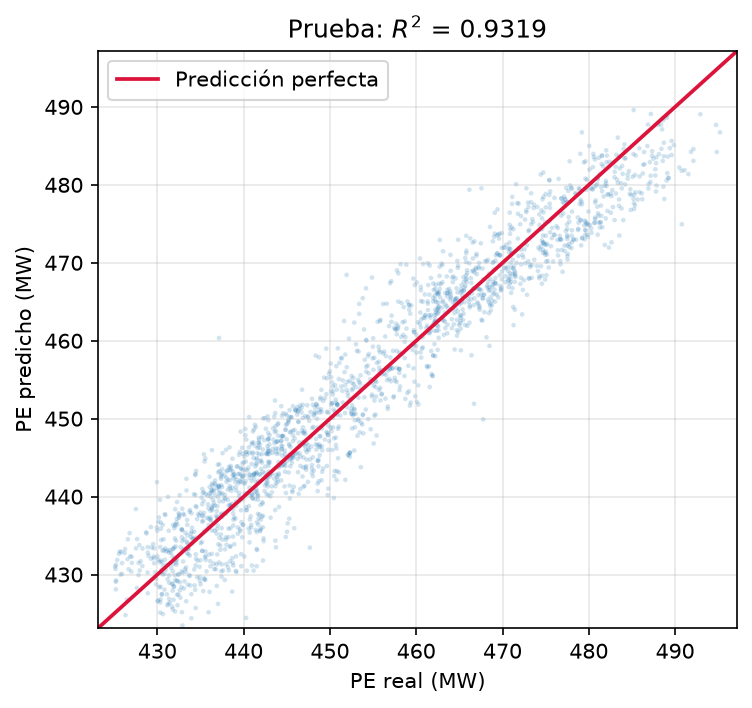
\includegraphics[width=\columnwidth]{figures/ajuste.png}
\caption{Valores predichos frente a valores reales en el conjunto de prueba.}
\label{fig:ajuste}
\end{figure}
\begin{figure}[htbp]
\centering
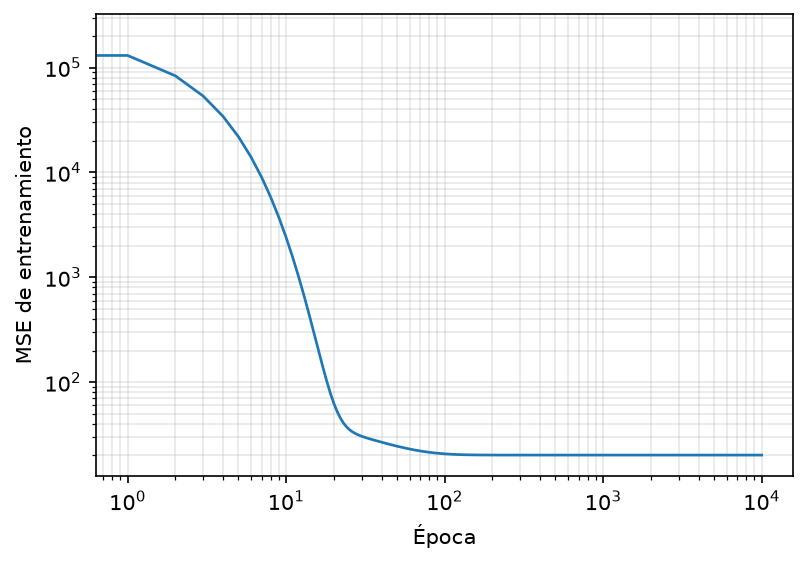
\includegraphics[width=\columnwidth]{figures/perdida.png}
\caption{Evolución del MSE de entrenamiento por época (ejes logarítmicos).}
\label{fig:perdida}
\end{figure}

\section{Diagnóstico del modelo}
\label{sec:diagnostico}
Los coeficientes de determinación de los tres sets están muy cerca entre sí: 0.9306 en entrenamiento, 0.9184 en validación y 0.9319 en prueba. La brecha entre entrenamiento y prueba es de menos de un punto porcentual, lo cual indica varianza baja y nada de sobreajuste, es decir, el modelo se comporta sobre datos que nunca vio prácticamente igual que sobre los datos con los que se ajustó. Esto es lo esperado considerando que el modelo estima solo 5 parámetros a partir de 5,716 observaciones de entrenamiento.

La validación cruzada de 5 particiones de la Tabla~\ref{tab:cv} confirma que el resultado no depende de la partición particular: un $R^2$ de $0.9283 \pm 0.0020$, una desviación lo suficientemente pequeña como para que cualquier otra partición diera prácticamente la misma cifra.

La Tabla~\ref{tab:cv} también muestra que un Random Forest alcanza un $R^2$ de 0.9616 contra 0.9283 del modelo lineal, sobre los mismos datos y las mismas particiones. Un árbol de decisión de profundidad 3, en cambio, se queda por debajo del modelo lineal con 0.9075: al tener solo 8 hojas únicamente puede devolver 8 valores distintos, y PE es una variable continua. La conclusión es que la relación entre las variables ambientales y la salida es predominantemente lineal, lo cual justifica el modelo elegido, pero no es exactamente lineal, y un modelo con suficiente flexibilidad encuentra la estructura que queda.

\begin{table}[htbp]
\caption{Validación cruzada de 5 particiones sobre el conjunto completo}
\label{tab:cv}
\centering
\begin{tabular}{lcc}
\toprule
Modelo & RMSE (media $\pm$ desv.) & $R^2$ (media $\pm$ desv.) \\
\midrule
Regresión lineal & $4.5603 \pm 0.0628$ & $0.9283 \pm 0.0020$ \\
Árbol (profundidad 3) & $5.1801 \pm 0.0565$ & $0.9075 \pm 0.0026$ \\
Random Forest & $3.3395 \pm 0.0993$ & $0.9616 \pm 0.0019$ \\
\bottomrule
\end{tabular}
\end{table}

\section{Comparación con framework}
\label{sec:comparacion}
Para validar la implementación, se entrenó un modelo con la clase \texttt{LinearRegression} de scikit-learn sobre el mismo set de entrenamiento y se evaluó sobre el mismo set de pruebas. La Tabla~\ref{tab:comparacion} compara los dos.

Las dos soluciones coinciden hasta el cuarto decimal en los cuatro coeficientes, en el intercepto y en el coeficiente de determinación. La razón es que las dos llegan al mismo punto por caminos diferentes: con el error cuadrático medio solo existe un punto donde el costo es mínimo, entonces no hay otro lugar al que cualquiera de las dos pudiera llegar. El gradiente descendente llega ahí de manera iterativa después de suficientes épocas, mientras que los mínimos cuadrados ordinarios de scikit-learn lo obtienen directo resolviendo las ecuaciones normales en forma cerrada.

Que coincidan también valida la conversión de los coeficientes descrita en la sección~\ref{sec:transformaciones}, ya que el modelo manual se entrenó con datos estandarizados y scikit-learn con las unidades originales, y los coeficientes solo pueden coincidir si la conversión de regreso está bien hecha.

La diferencia entre las dos implementaciones no está entonces en el resultado sino en lo que cuesta llegar a él. El modelo manual necesita 10,000 iteraciones sobre 5,716 observaciones y unos 30 segundos de cómputo, mientras que la solución cerrada se obtiene en un solo paso. Aun así, el método iterativo es el que escala a modelos que no tienen solución cerrada, y por eso es la base del entrenamiento de prácticamente todos los modelos modernos de machine learning.

\begin{table}[htbp]
\caption{Modelo manual vs scikit-learn (unidades originales)}
\label{tab:comparacion}
\centering
\begin{tabular}{lccc}
\toprule
Parámetro & Manual (GD) & scikit-learn (OLS) & Diferencia \\
\midrule
$\beta_{AT}$ & $-1.9819$ & $-1.9819$ & 0 \\
$\beta_{V}$ & $-0.2374$ & $-0.2374$ & 0 \\
$\beta_{AP}$ & 0.0555 & 0.0555 & 0 \\
$\beta_{RH}$ & $-0.1592$ & $-0.1592$ & 0 \\
$b$ & 461.6212 & 461.6212 & 0 \\
$R^2$ prueba & 0.9319 & 0.9319 & 0 \\
\bottomrule
\end{tabular}
\end{table}

\section{Ajuste de hiperparámetros}
\label{sec:hiperparametros}
El efecto de los dos hiperparámetros se midió sobre el set de validación, dejando el set de pruebas sin tocar hasta que la configuración ya estaba elegida.

La Tabla~\ref{tab:lr} muestra el efecto de la tasa de aprendizaje con un presupuesto fijo de 2,000 épocas, y la Figura~\ref{fig:lrsweep} las curvas de convergencia correspondientes. Con $\alpha = 0.001$ los pasos son tan pequeños que después de 2,000 épocas el modelo sigue lejos del mínimo, con un error de entrenamiento de 3,775.77 y un coeficiente de determinación negativo, es decir, predice peor que simplemente usar el promedio de los datos. De $\alpha = 0.05$ en adelante todas las tasas llegan al mismo mínimo de 20.147, porque el punto mínimo es siempre el mismo y el tamaño del paso no cambia a dónde se llega, solo cuántas iteraciones hacen falta para llegar. Con $\alpha = 0.9$ cada paso se pasa de largo del mínimo y amplifica el error en lugar de reducirlo, entonces los valores se salen del rango de los números flotantes y el entrenamiento diverge.

La Tabla~\ref{tab:epocas} muestra el efecto del número de épocas con la tasa automática. A las 100 épocas el modelo ya está prácticamente convergido, con un $R^2$ de 0.9170 contra el 0.9184 que alcanza de las 500 en adelante, y más allá de ese punto las iteraciones adicionales no cambian nada. Esto confirma que no hay ninguna penalización por iterar más de lo necesario: el modelo no se sobreajusta por entrenar más épocas, simplemente deja de mejorar. Las 10,000 épocas del caso base dan entonces un buen margen de seguridad a un costo de unos cuantos segundos.

Los dos resultados apuntan a lo mismo: con los datos estandarizados la tasa automática cae dentro del rango que converge y la elección del número de épocas deja de ser crítica.

\begin{table}[htbp]
\caption{Efecto de la tasa de aprendizaje (2\,000 épocas)}
\label{tab:lr}
\centering
\begin{tabular}{lccc}
\toprule
$\alpha$ & MSE final entren. & RMSE val. & $R^2$ val. \\
\midrule
0.001 & 3775.768 & 61.579 & $-11.9832$ \\
0.01 & 20.722 & 4.927 & 0.9169 \\
0.05 & 20.147 & 4.881 & 0.9184 \\
auto (0.2) & 20.147 & 4.881 & 0.9184 \\
0.5 & 20.147 & 4.881 & 0.9184 \\
0.9 & diverge & --- & --- \\
\bottomrule
\end{tabular}
\end{table}

\begin{table}[htbp]
\caption{Efecto del número de épocas ($\alpha$ automática)}
\label{tab:epocas}
\centering
\begin{tabular}{lccc}
\toprule
Épocas & MSE entren. & MSE val. & $R^2$ val. \\
\midrule
100 & 20.698 & 24.251 & 0.9170 \\
500 & 20.147 & 23.825 & 0.9184 \\
1\,000 & 20.147 & 23.825 & 0.9184 \\
2\,000 & 20.147 & 23.825 & 0.9184 \\
5\,000 & 20.147 & 23.825 & 0.9184 \\
10\,000 & 20.147 & 23.825 & 0.9184 \\
\bottomrule
\end{tabular}
\end{table}

\begin{figure}[htbp]
\centering
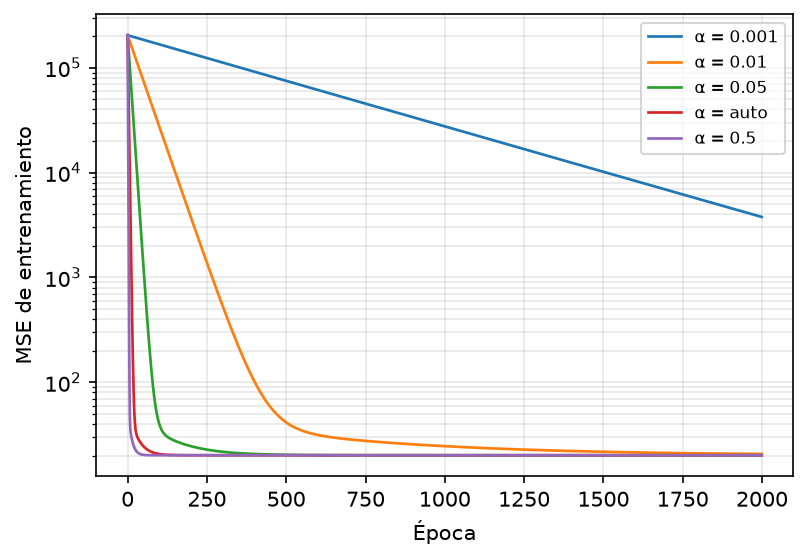
\includegraphics[width=\columnwidth]{figures/lr_sweep.png}
\caption{Convergencia del MSE de entrenamiento según la tasa de aprendizaje (2000 épocas; la curva divergente se omite).}
\label{fig:lrsweep}
\end{figure}

\section{Conclusiones}
\label{sec:conclusiones}
Se implementó desde cero un modelo de regresión lineal múltiple entrenado con gradiente descendente, sin frameworks de machine learning, y se validó sobre un dataset real de 9,527 registros por hora de una planta de ciclo combinado. El modelo explica el 93.19\% de la varianza del set de pruebas, con un RMSE de 4.43 MW, y alcanza coeficientes idénticos a los de scikit-learn hasta el cuarto decimal, lo cual confirma que la implementación es correcta.

El hallazgo práctico más importante es que la estandarización de las variables no es un paso cosmético sino la condición que hace viable el modelo. La heurística que estima la tasa de aprendizaje a partir de la escala de los datos funciona bien cuando todas las features comparten una escala, pero sobre los datos originales una sola variable con unidades grandes, la presión ambiente con valores alrededor de 1013, domina el cálculo y produce una tasa de 0.00000097, tan pequeña que el modelo no converge en un número práctico de épocas.

El diagnóstico también muestra los límites del modelo. Un Random Forest entrenado con los mismos datos alcanza un $R^2$ de 0.9616 contra el 0.9283 del modelo lineal. La relación entre las variables ambientales y la salida de potencia es entonces predominantemente lineal, pero no exactamente lineal.

El modelo no tiene regularización, que aquí no hizo falta por la varianza baja que se observó, pero sí haría falta con más features o menos observaciones. Tampoco incluye términos de interacción ni polinómicos, que es de donde probablemente viene la ventaja del Random Forest. Agregar términos cuadráticos para la temperatura ambiente, o una interacción entre la temperatura y el vacío de escape, que son las dos variables más correlacionadas entre sí, es la extensión más directa de este trabajo, y permitiría ver cuánto de esa ventaja se puede recuperar sin abandonar un modelo lineal.

\begin{thebibliography}{00}
\bibitem{b1} G. James, D. Witten, T. Hastie y R. Tibshirani, \textit{An Introduction to Statistical Learning}. Springer, 2021.
\bibitem{b2} I. Goodfellow, Y. Bengio y A. Courville, \textit{Deep Learning}. MIT Press, 2016.
\bibitem{b3} P. Tüfekci, ``Prediction of full load electrical power output of a base load operated combined cycle power plant using machine learning methods,'' \textit{International Journal of Electrical Power \& Energy Systems}, vol. 60, pp. 126--140, 2014.
\bibitem{b4} Combined Cycle Power Plant, UCI Machine Learning Repository: \url{https://archive.ics.uci.edu/dataset/294/combined+cycle+power+plant}
\bibitem{b5} Repositorio del proyecto: \url{https://github.com/Facundo-Barbera/linear-regression-from-scratch}
\end{thebibliography}

\end{document}
